\chapter{Resultados} \label{chap:resultados} % ### 7.

Neste capítulos serão apresentados os resultados obtidos com a \hyperref[sec:sistema]{implementação do sistema} de gerenciamento de suporte à decisão discutido ao longo deste trabalho. Serão apresentadas as \hyperref[ssec:paginas]{páginas} desenvolvidas, bem como as \hyperref[ssec:funcionalidades]{funcionalidades} implementadas.

% \section{UENF}

% \section{Entrevistas}

% \section{Formulário}

\section{Sistema desenvolvido} \label{sec:sistema}

O sistema foi desenvolvido utilizando a linguagem de programação JavaScript em conjunto com o React, um framework de desenvolvimento de interfaces de usuário. O sistema consiste de um conjunto de \hyperref[ssec:paginas]{oito páginas} principais, das quais emergem diversas \hyperref[ssec:funcionalidades]{funcionalidades}.

\subsection{Páginas} \label{ssec:paginas}

\autoref{fig:main}
\autoref{fig:multiFiltros}
\autoref{fig:multiConflitos}
\autoref{fig:multiDisciplinas}
\autoref{fig:grade}
\autoref{fig:turmas}
\autoref{fig:professores}
\autoref{fig:salas}
\autoref{fig:disciplinas}
\autoref{fig:alunos}

\begin{MyCenteredFigure} \caption{Página inicial do sistema} \label{fig:main}
  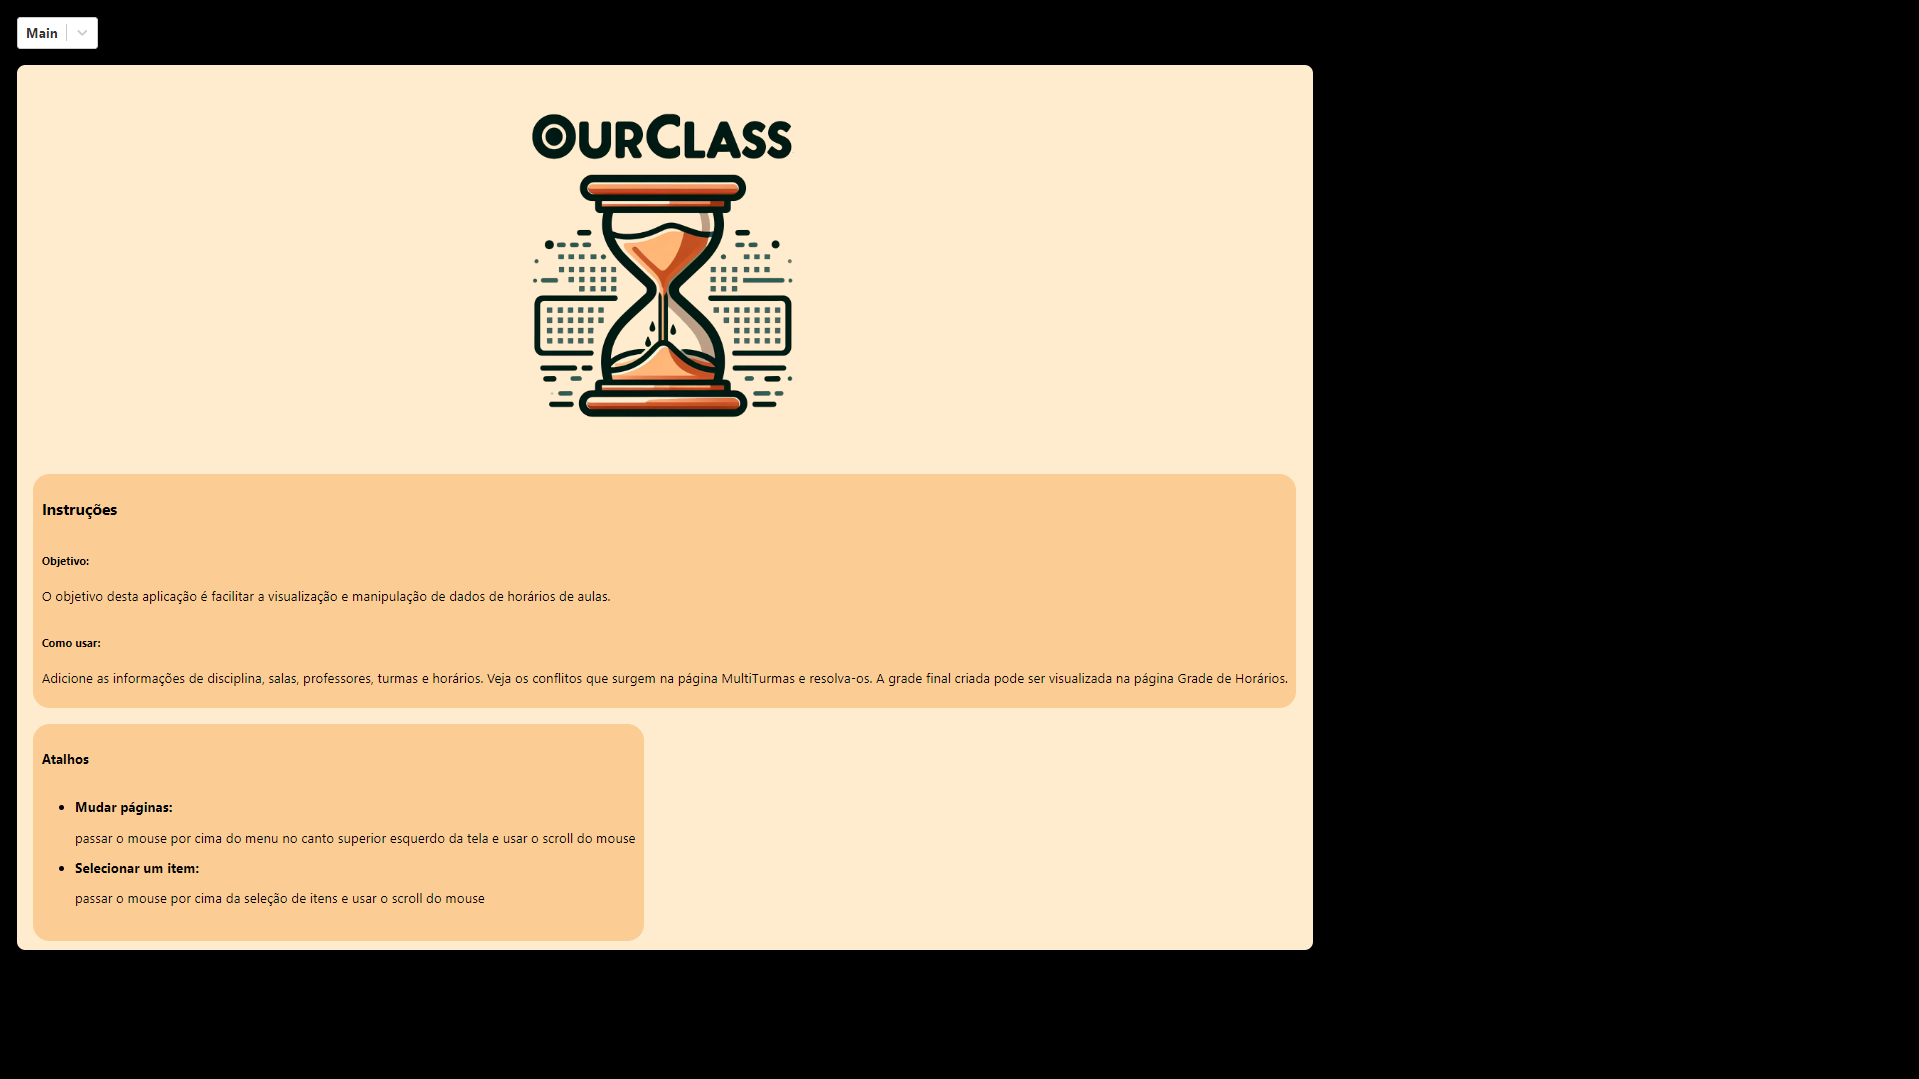
\includegraphics[width=\textwidth]{files/img/2.02!7-resultados/1-Main.png}
\end{MyCenteredFigure}

\begin{MyCenteredFigure} \caption{Página de multiturmas com filtros} \label{fig:multiFiltros}
  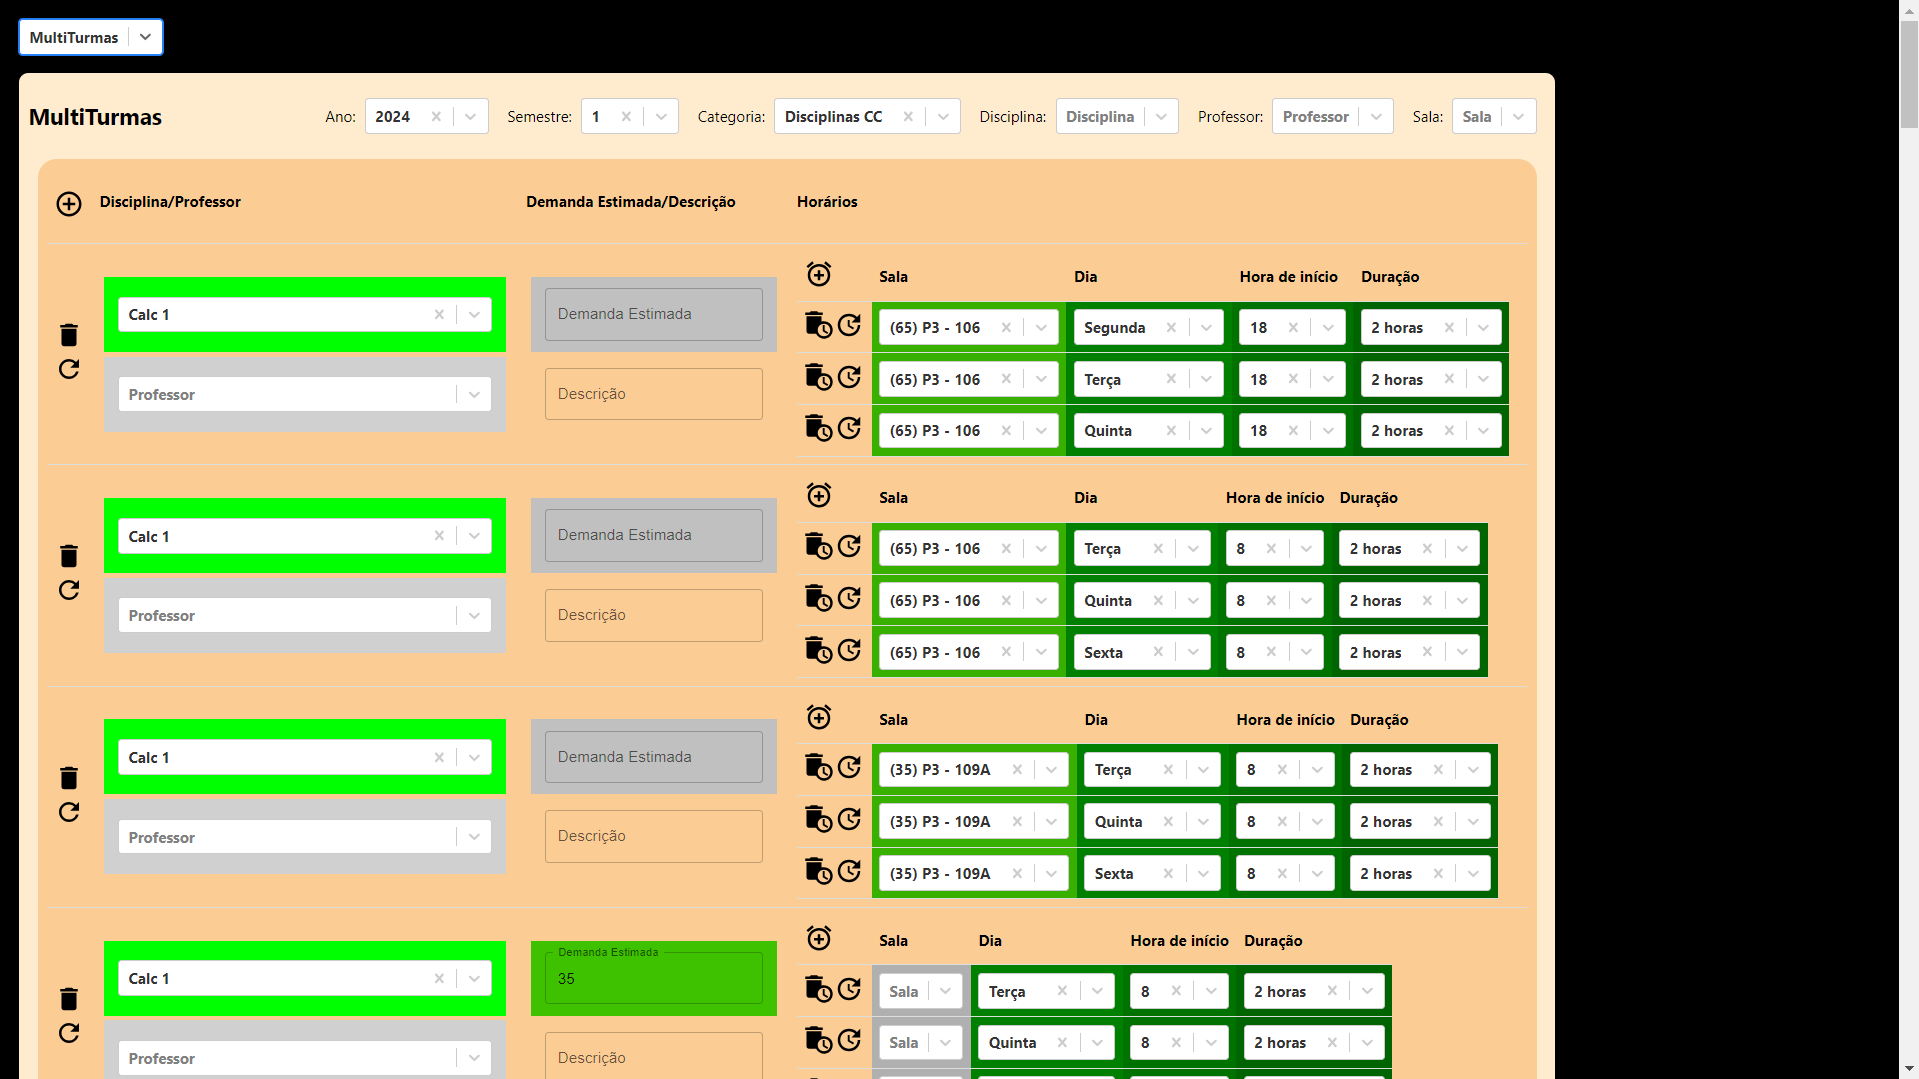
\includegraphics[width=\textwidth]{files/img/2.02!7-resultados/2-Multiturmas-Filtros.png}
\end{MyCenteredFigure}

\begin{MyCenteredFigure} \caption{Página de multiturmas com conflitos} \label{fig:multiConflitos}
  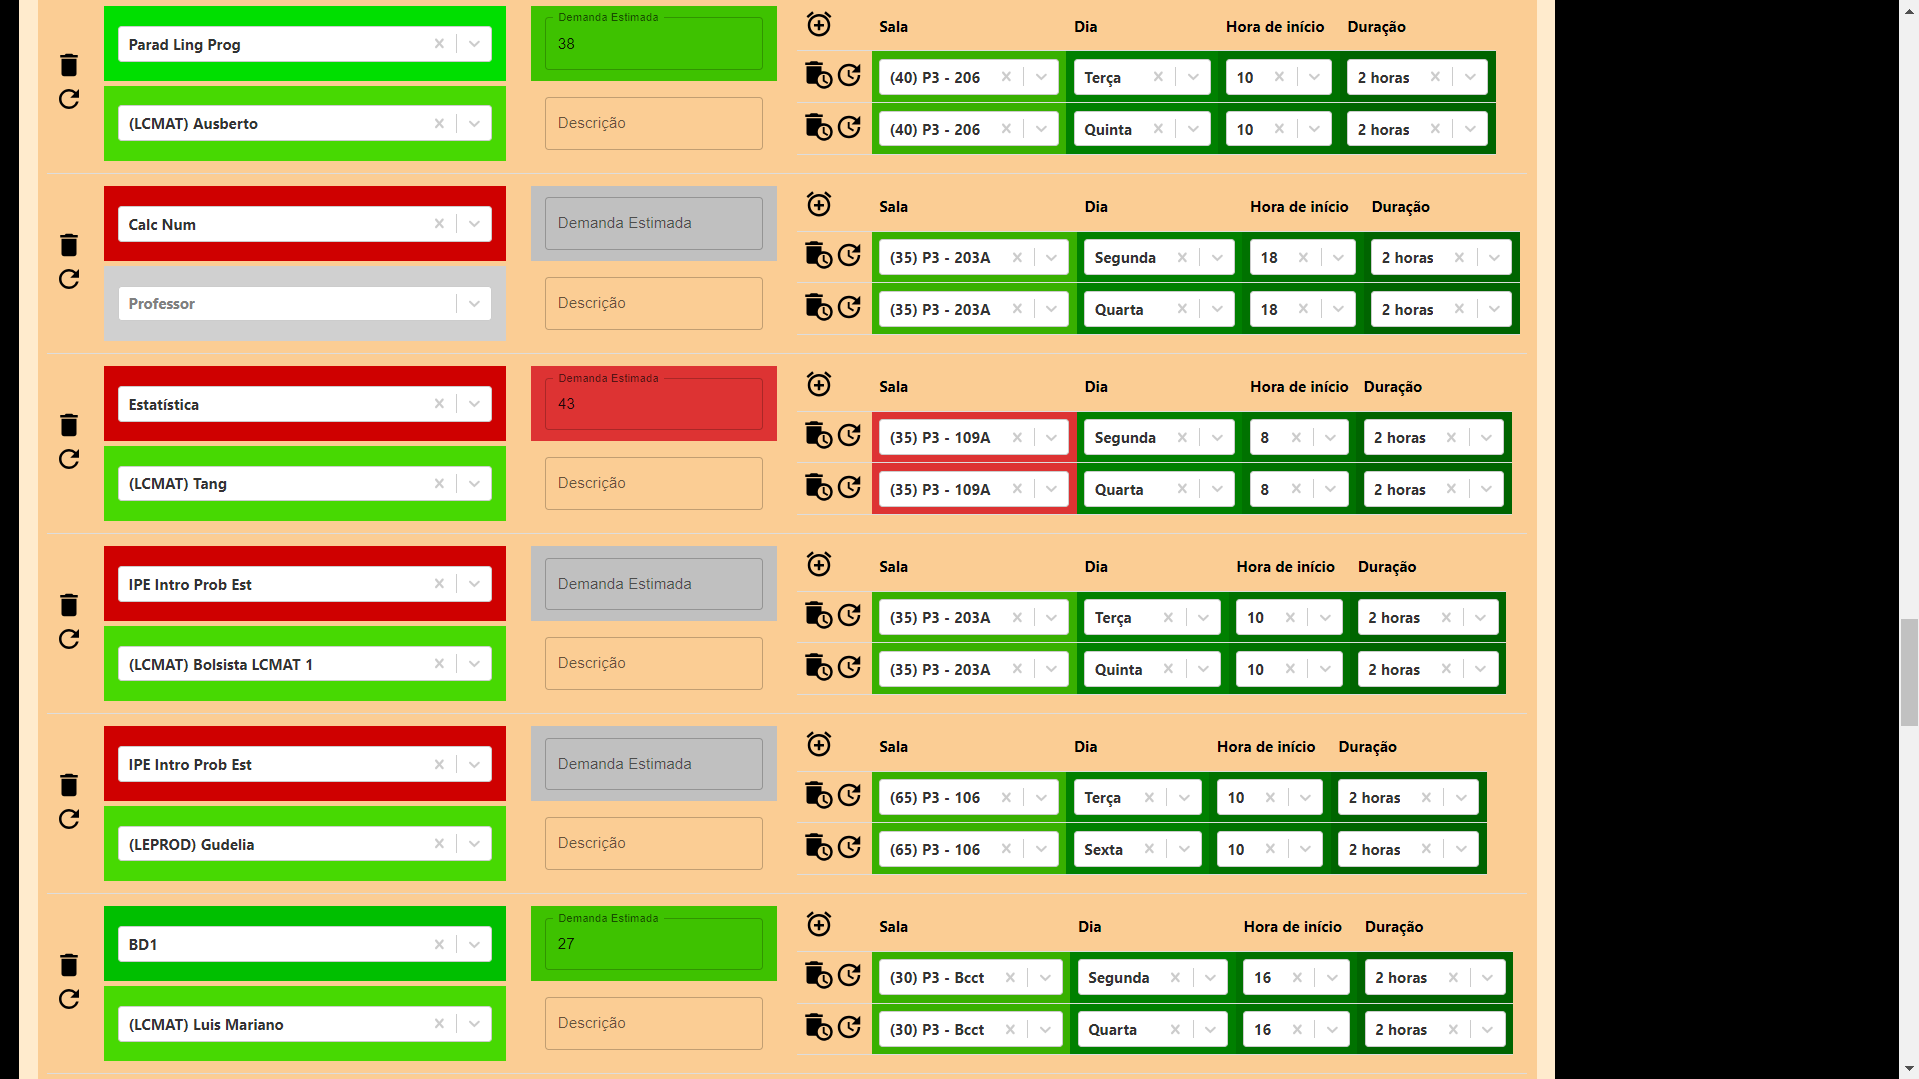
\includegraphics[width=\textwidth]{files/img/2.02!7-resultados/3-Multiturmas-Conflitos.png}
\end{MyCenteredFigure}

\begin{MyCenteredFigure} \caption{Página de multiturmas com disciplinas pendentes} \label{fig:multiDisciplinas}
  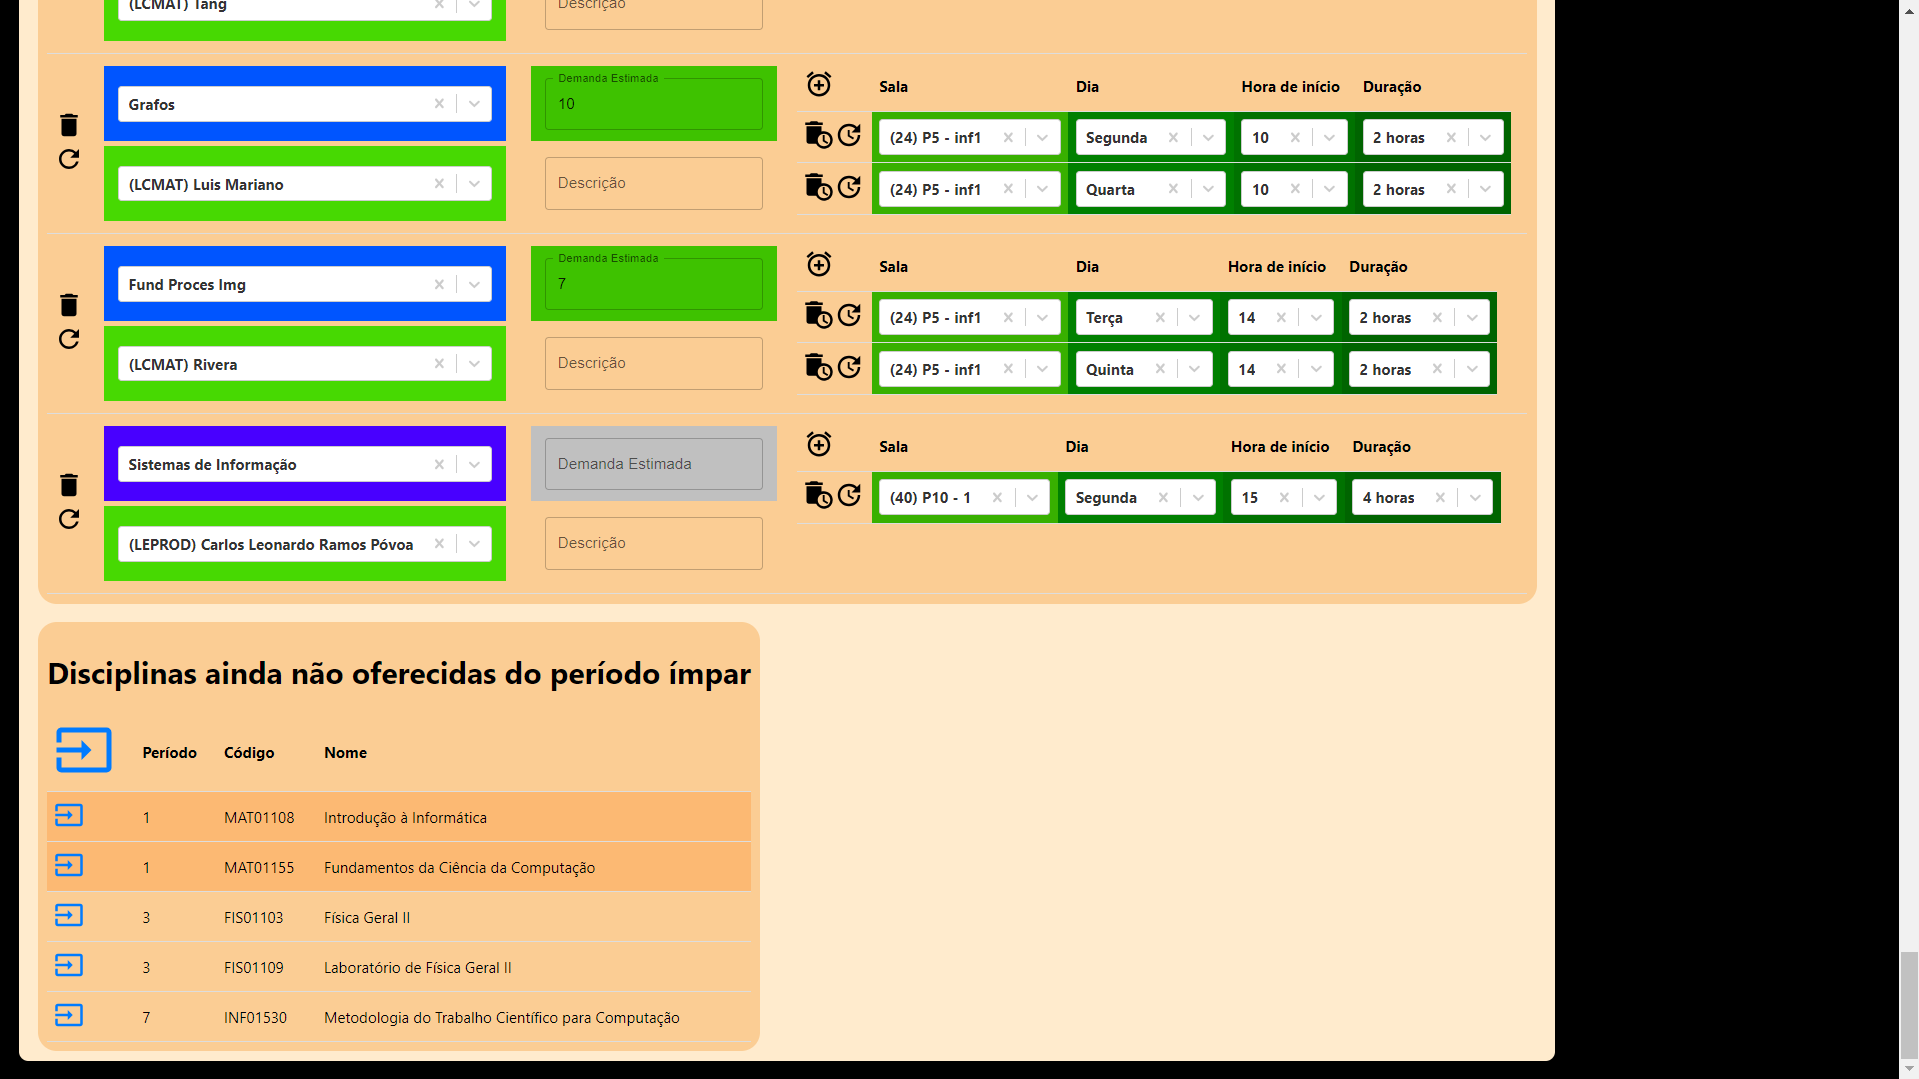
\includegraphics[width=\textwidth]{files/img/2.02!7-resultados/4-Multiturmas-DisciplinasPendentes.png}
\end{MyCenteredFigure}

\begin{MyCenteredFigure} \caption{Página de grade de horários} \label{fig:grade}
  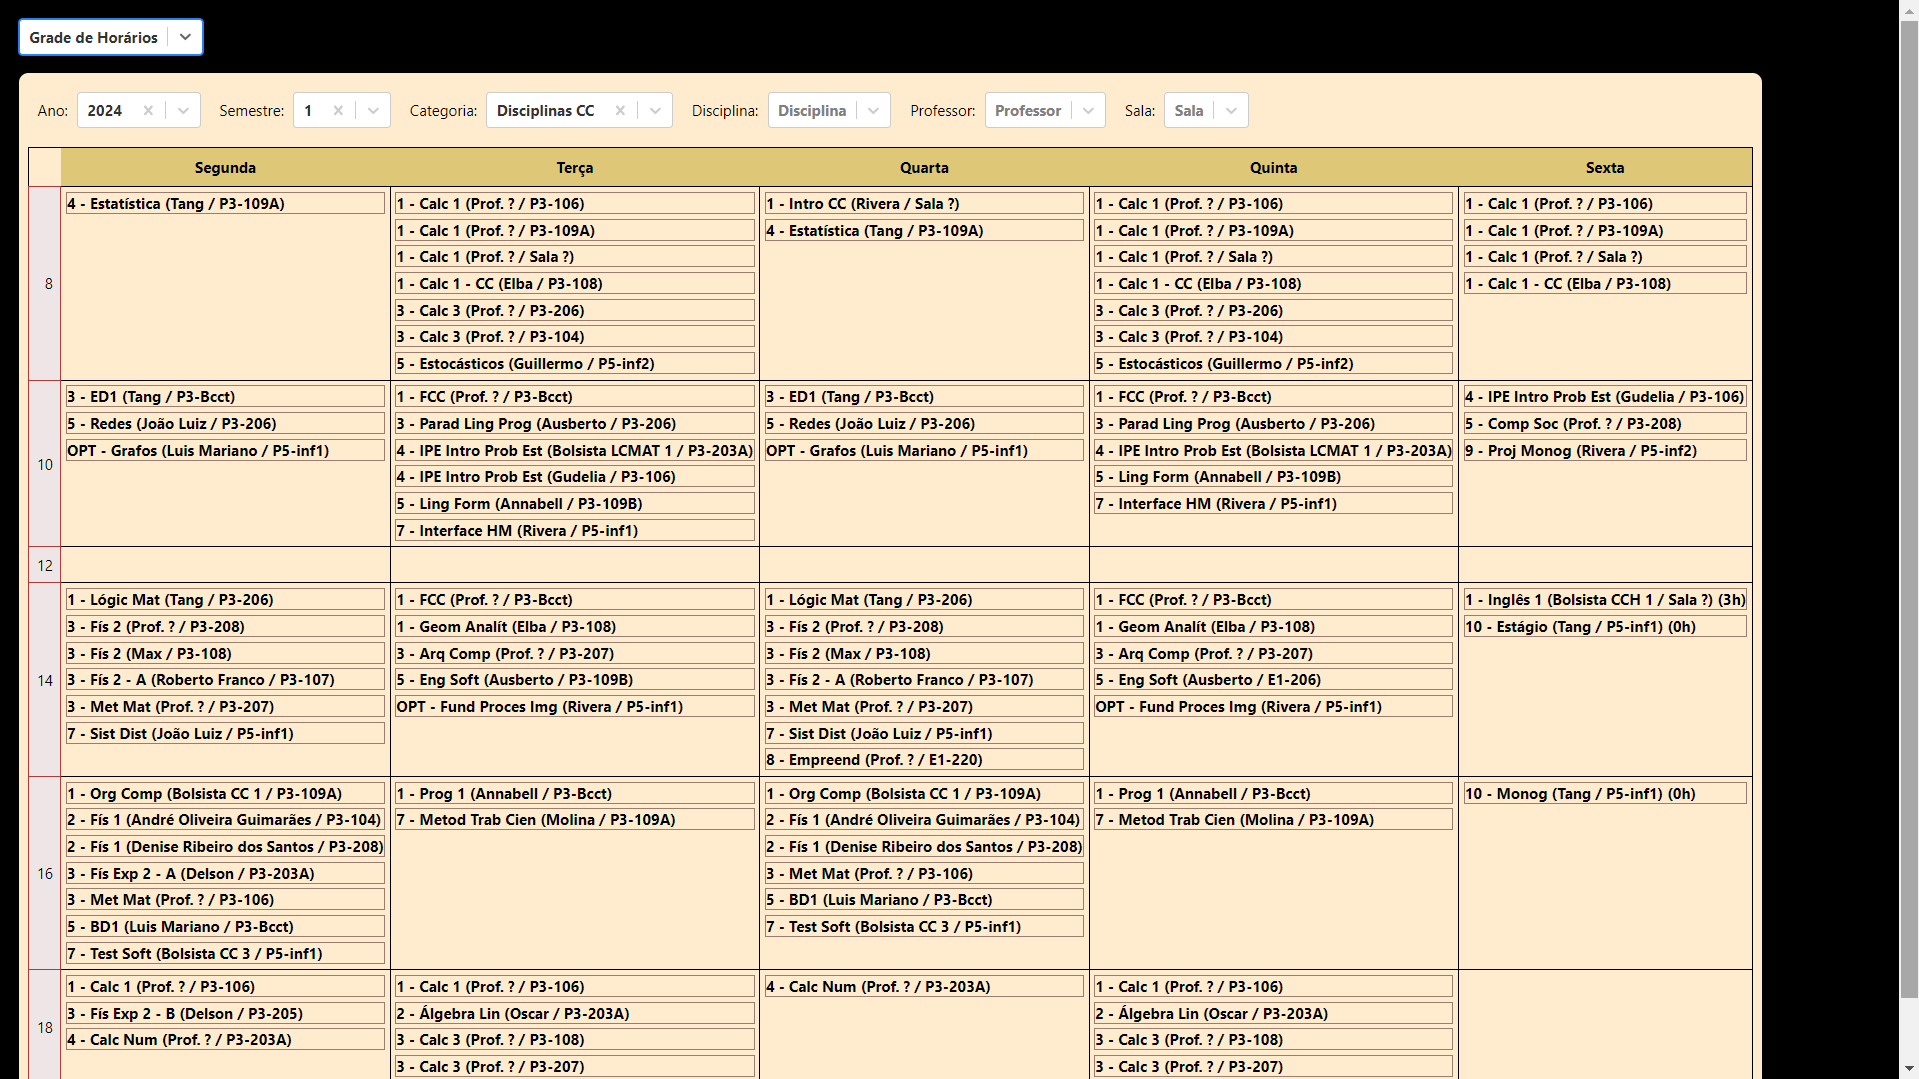
\includegraphics[width=\textwidth]{files/img/2.02!7-resultados/5-Grade de Horários.png}
\end{MyCenteredFigure}

\begin{MyCenteredFigure} \caption{Página de turmas} \label{fig:turmas}
  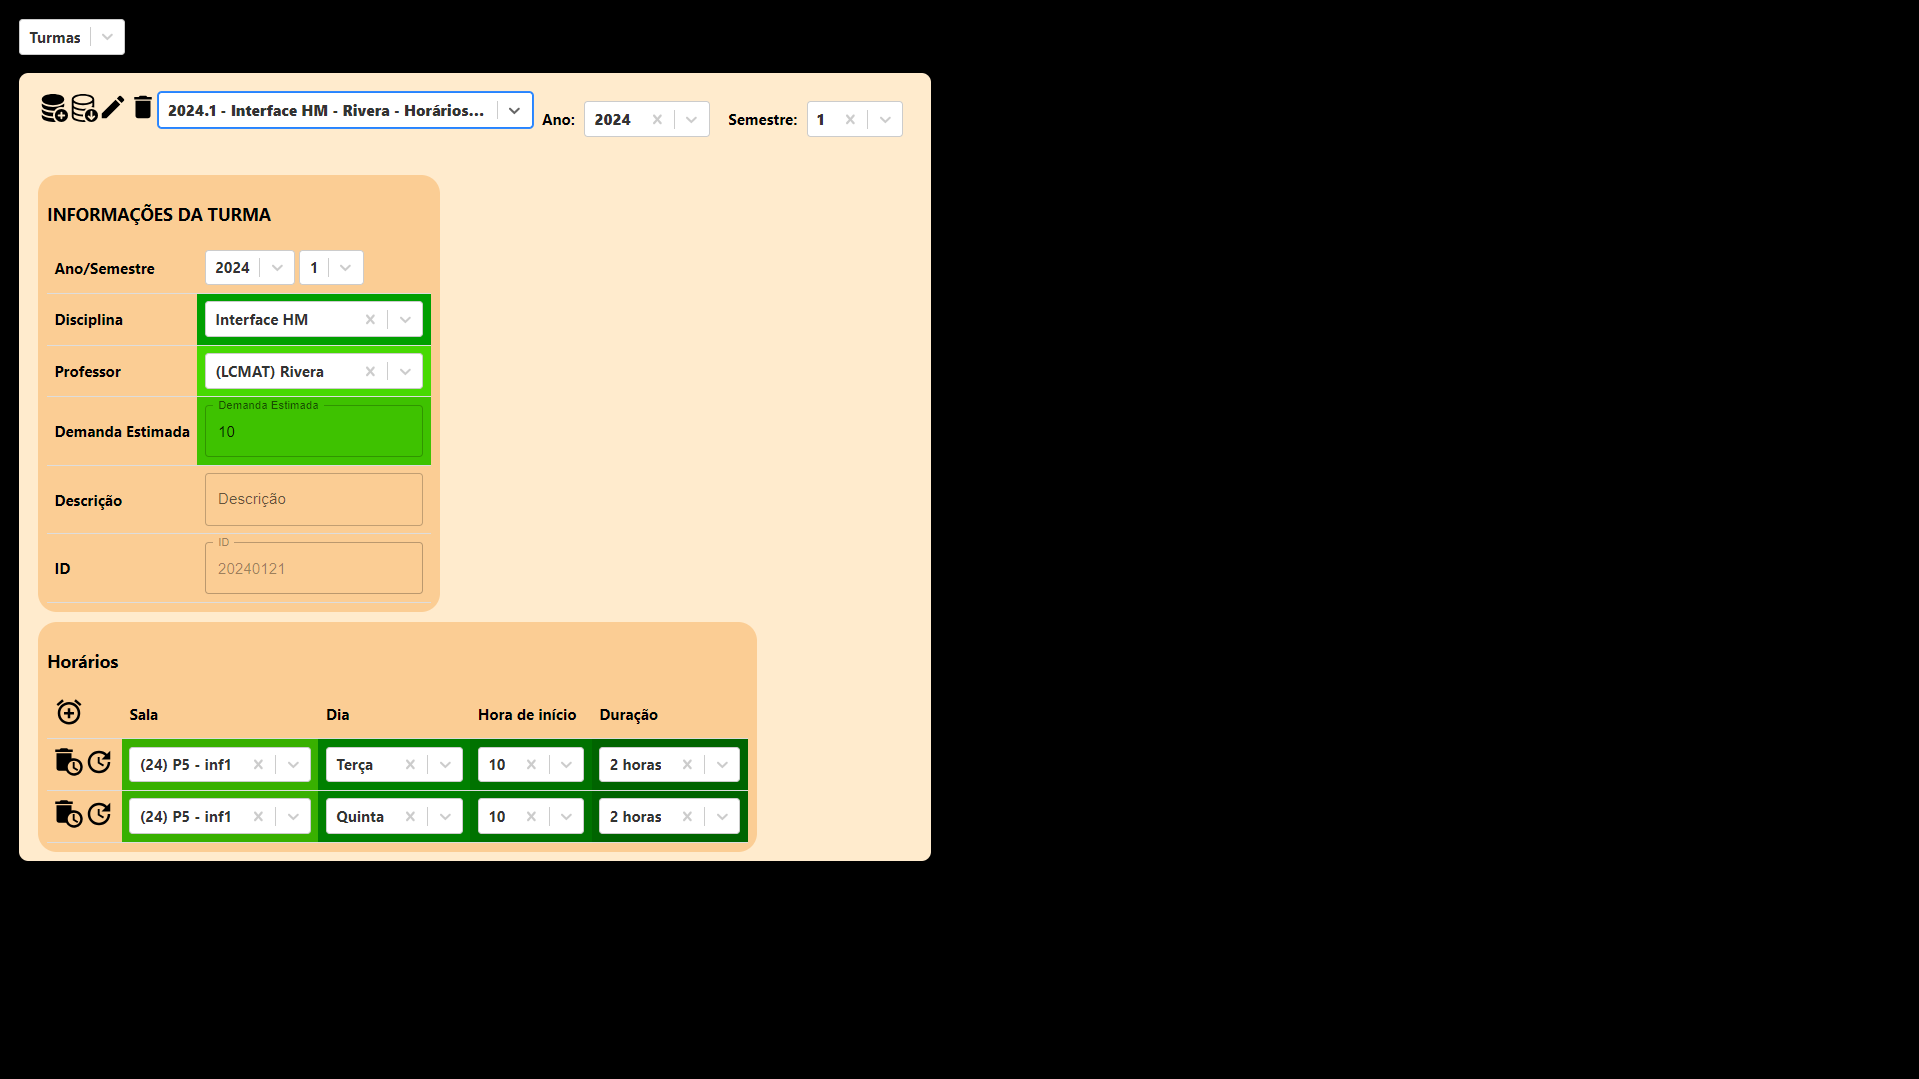
\includegraphics[width=\textwidth]{files/img/2.02!7-resultados/6-Turmas.png}
\end{MyCenteredFigure}

\begin{MyCenteredFigure} \caption{Página de professores} \label{fig:professores}
  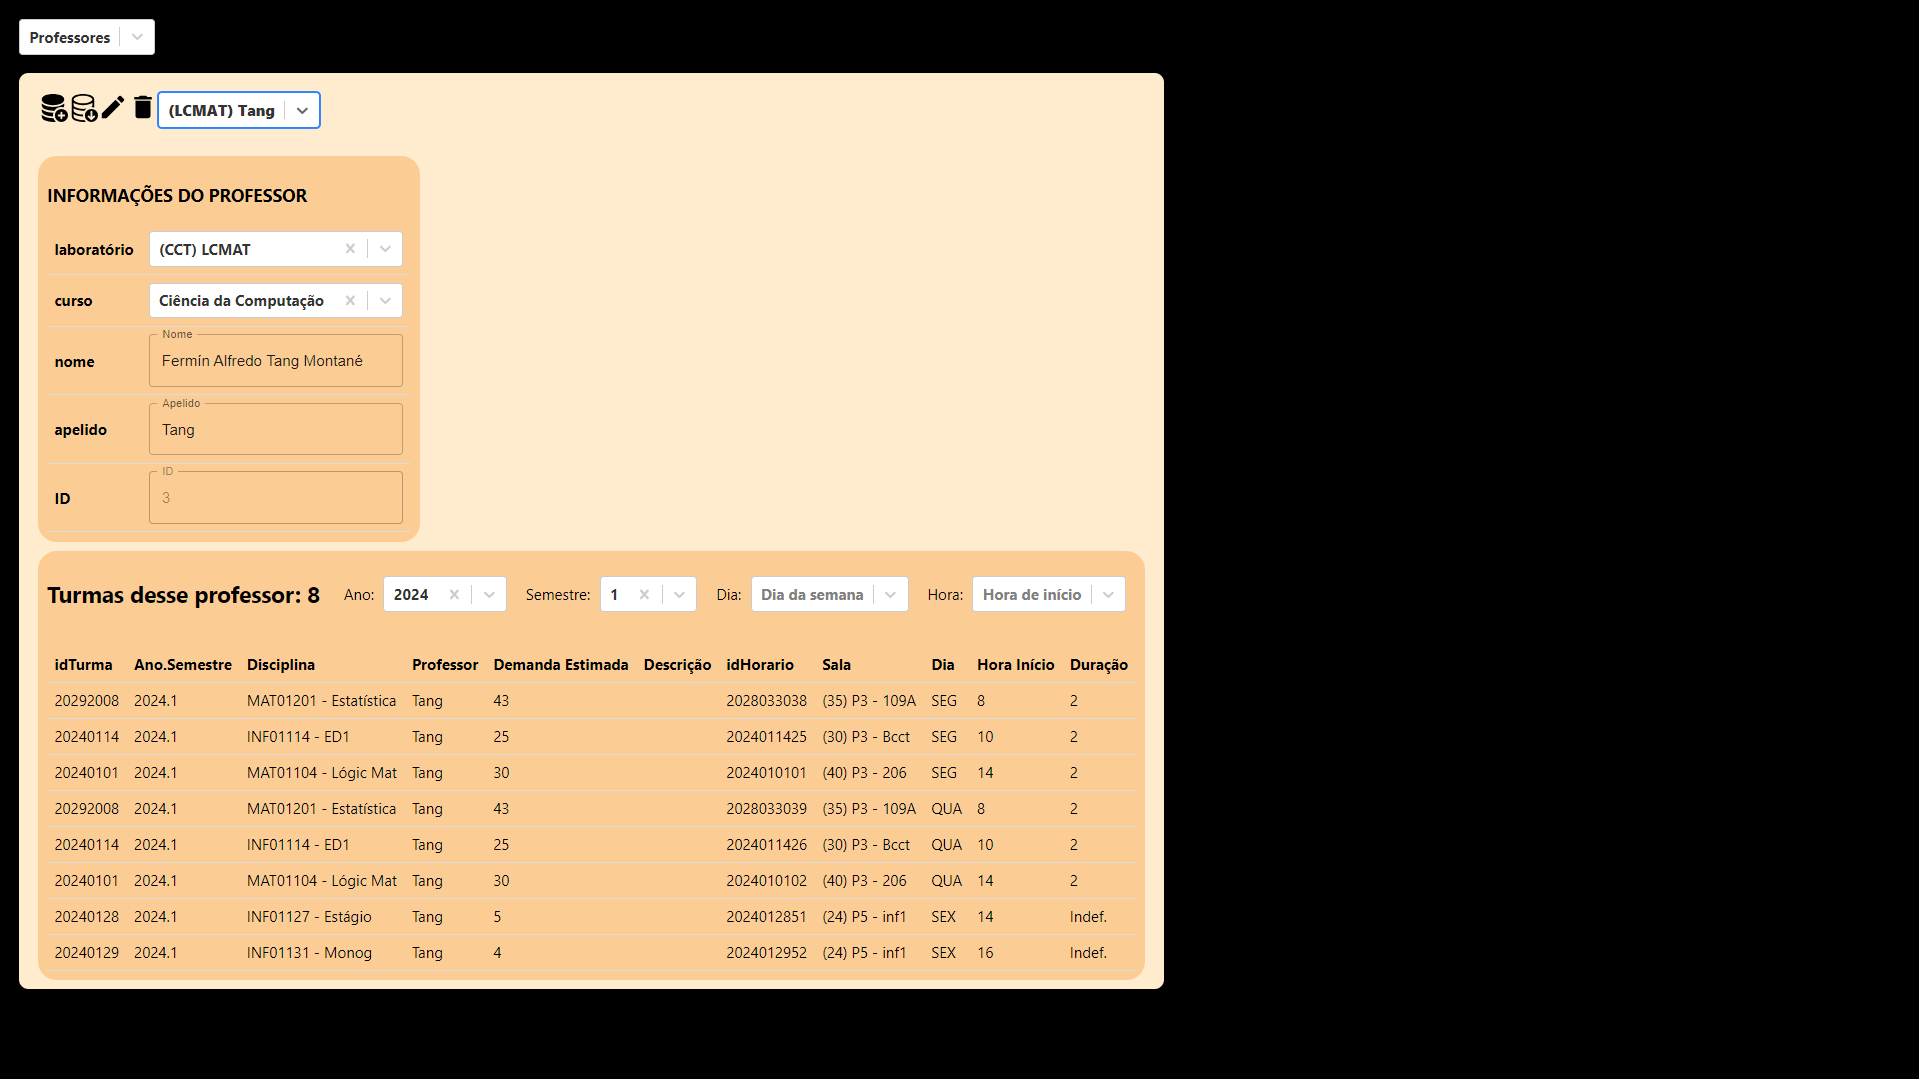
\includegraphics[width=\textwidth]{files/img/2.02!7-resultados/7-Professores.png}
\end{MyCenteredFigure}

\begin{MyCenteredFigure} \caption{Página de salas} \label{fig:salas}
  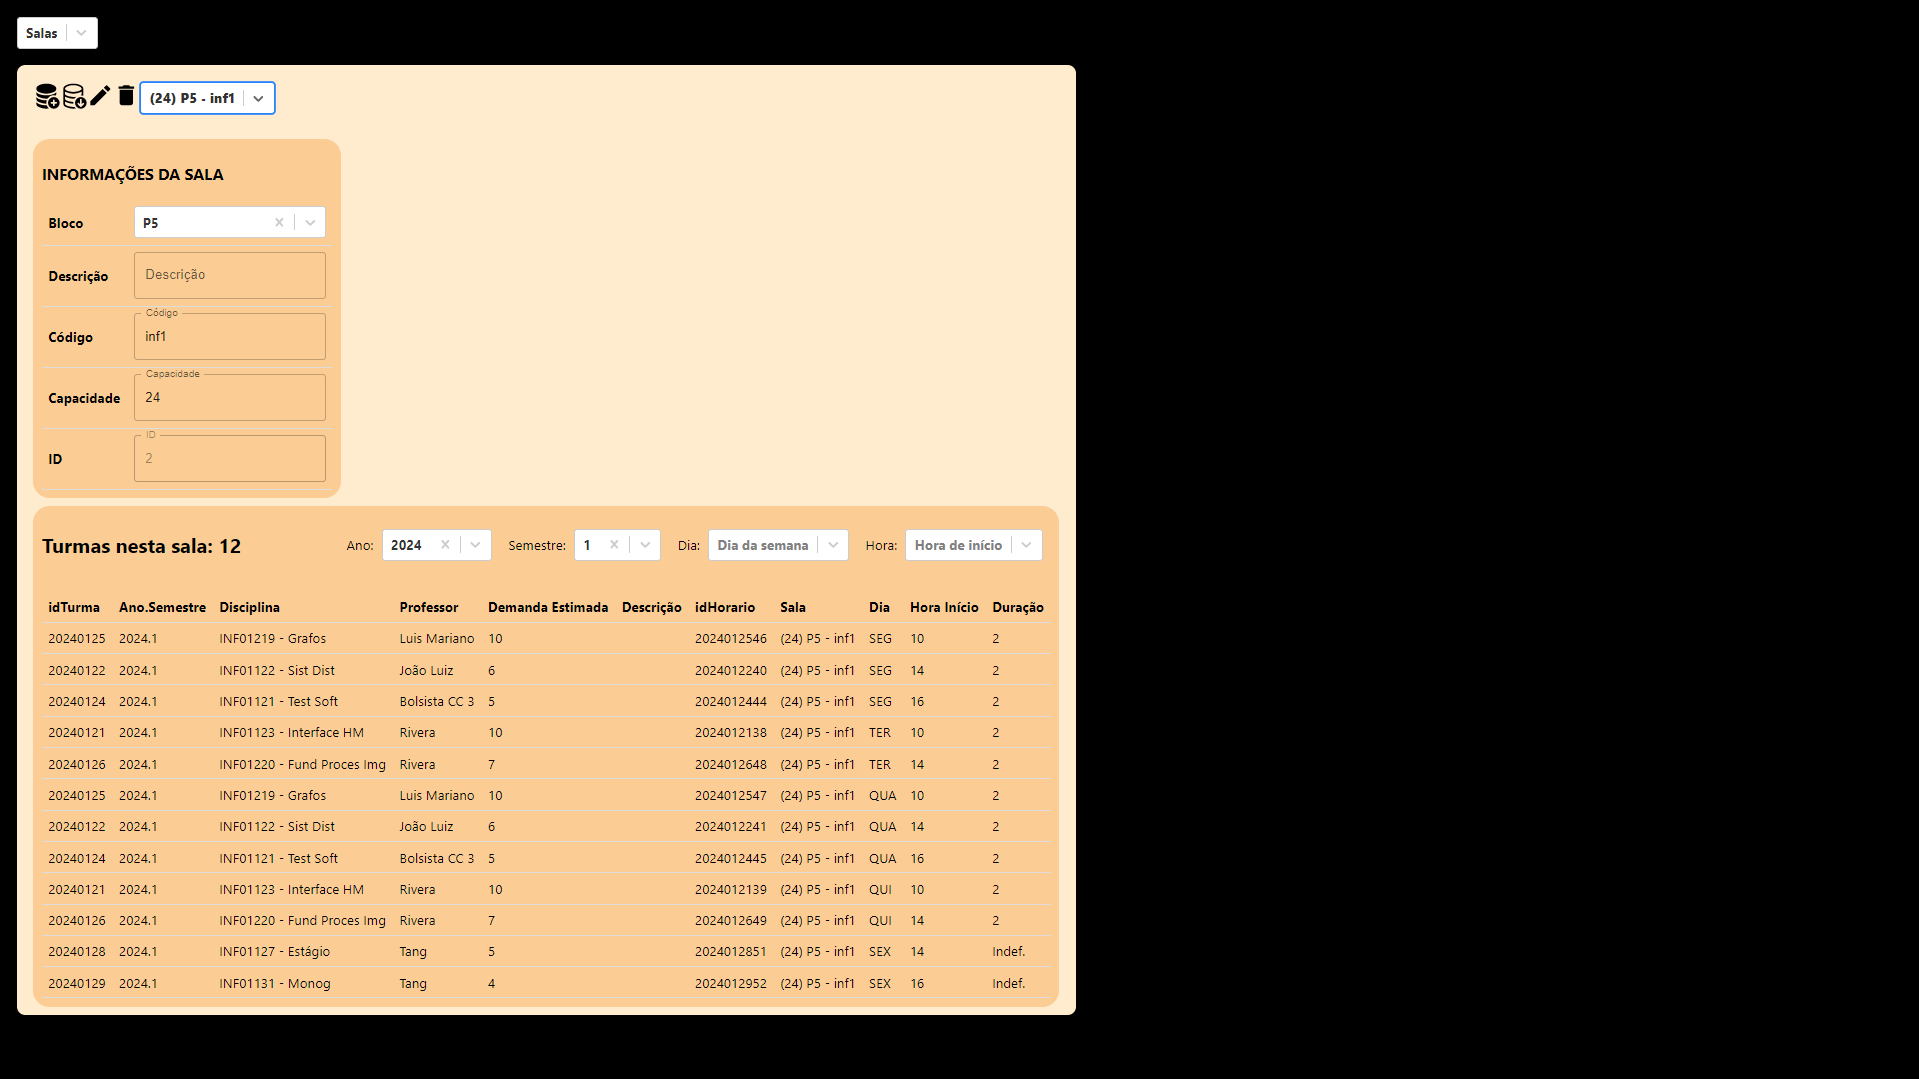
\includegraphics[width=\textwidth]{files/img/2.02!7-resultados/8-Salas.png}
\end{MyCenteredFigure}

\begin{MyCenteredFigure} \caption{Página de disciplinas} \label{fig:disciplinas}
  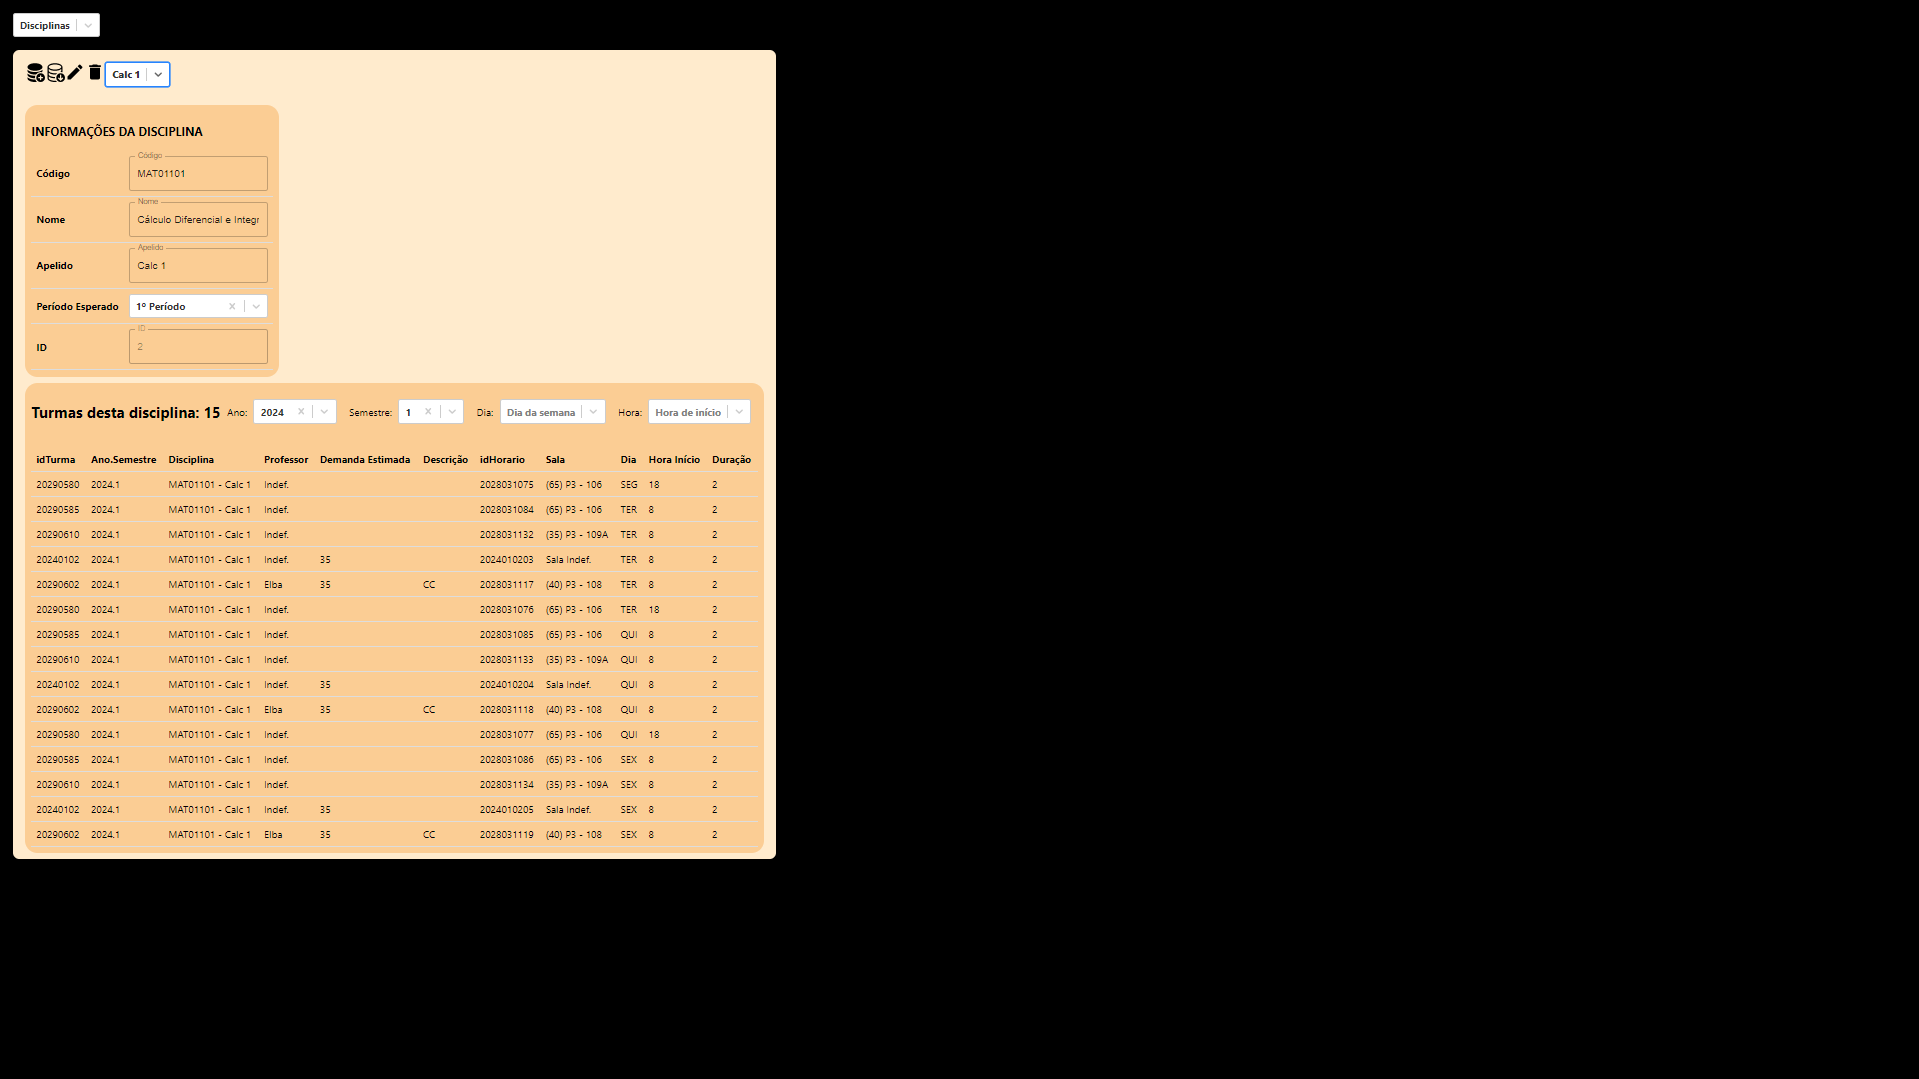
\includegraphics[width=\textwidth]{files/img/2.02!7-resultados/9-Disciplinas.png}
\end{MyCenteredFigure}

\begin{MyCenteredFigure} \caption{Página de alunos} \label{fig:alunos}
  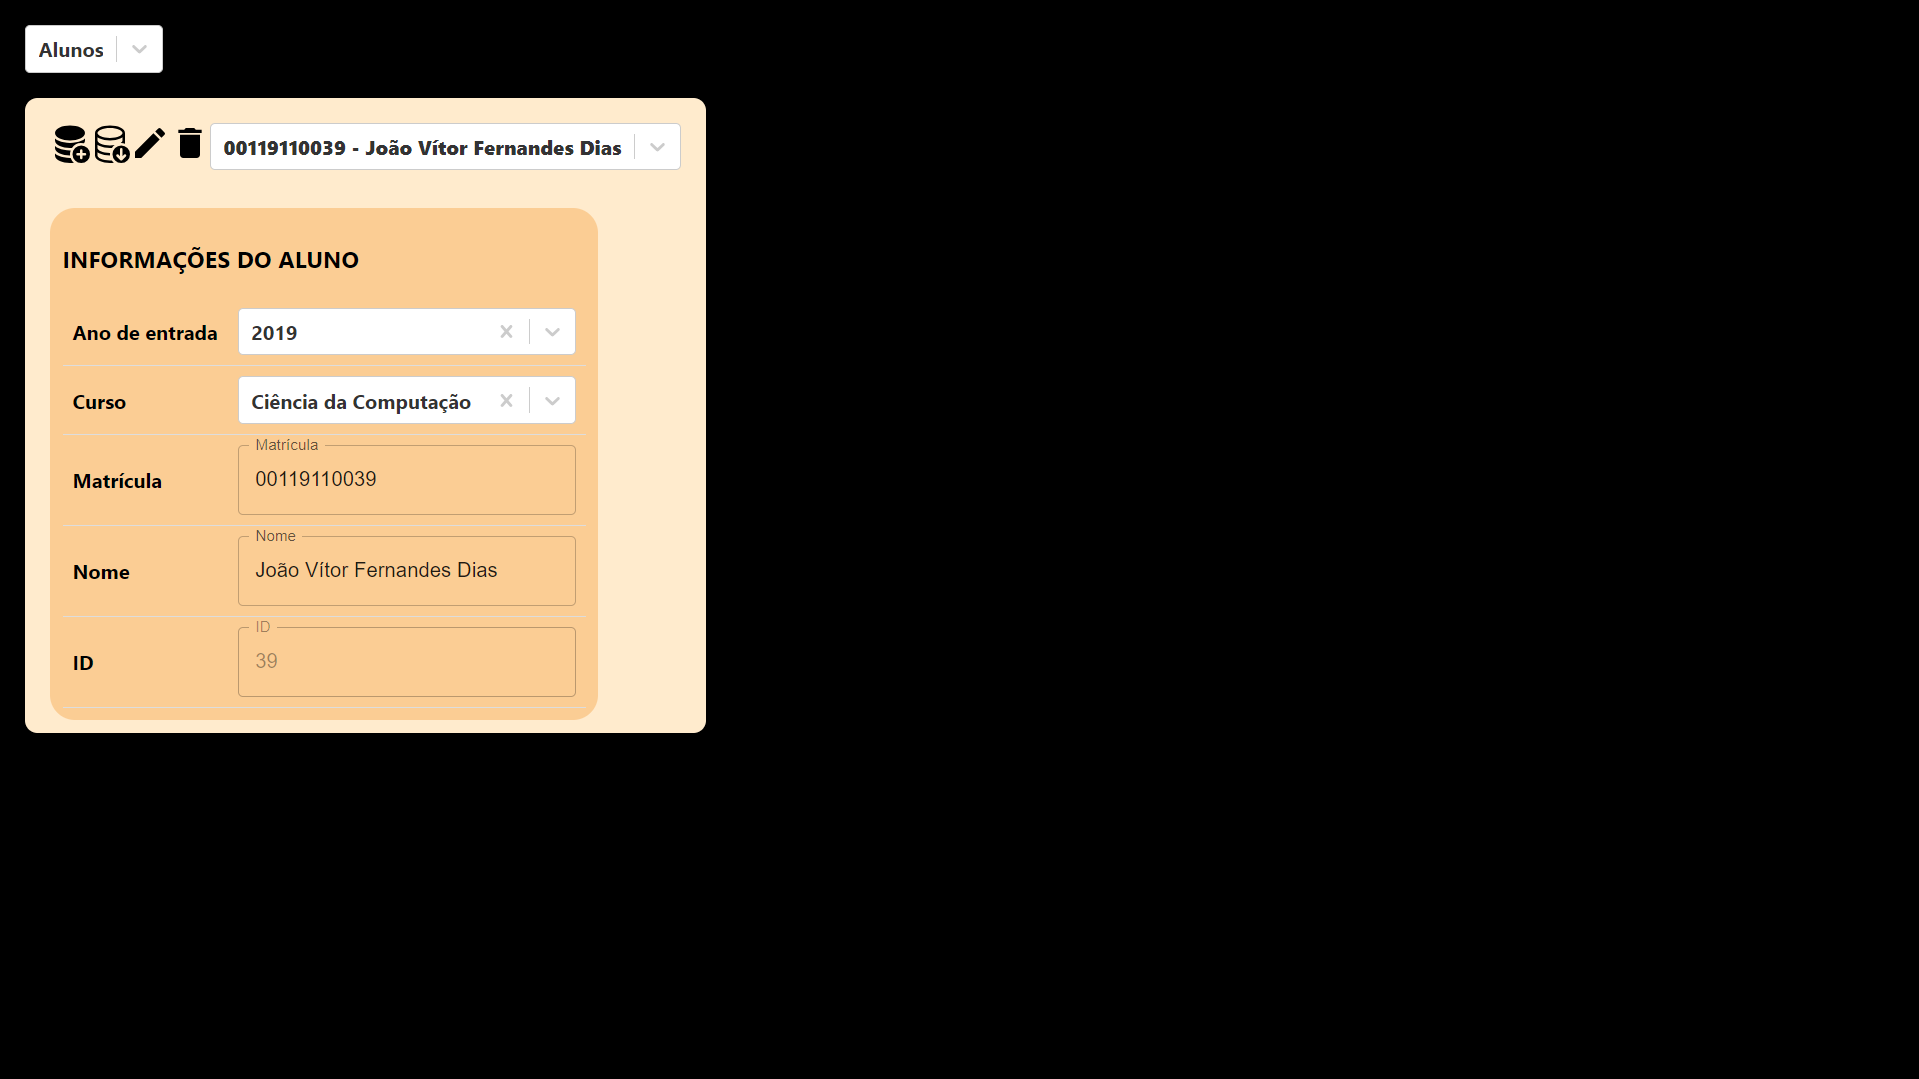
\includegraphics[width=\textwidth]{files/img/2.02!7-resultados/10-Aluno.png}
\end{MyCenteredFigure}

\subsection{Funcionalidades} \label{ssec:funcionalidades}

X funcionalidades principais, com hyperlinks

\hyperref[sssec:CRUD]{CRUD}
\hyperref[sssec:Análise histórica]{Análise histórica}
\hyperref[sssec:Criação de grade inicial]{Criação de grade inicial}
\hyperref[sssec:Visualização de conflitos]{Visualização de conflitos}
\hyperref[sssec:Visualização de tabelas horárias]{Visualização de tabelas horárias}


\subsubsection{CRUD} \label{sssec:CRUD}

\subsubsection{Análise histórica} \label{sssec:Análise histórica}

\subsubsection{Criação de grade inicial} \label{sssec:Criação de grade inicial}

\subsubsection{Visualização de conflitos} \label{sssec:Visualização de conflitos}

\subsubsection{Visualização de tabelas horárias} \label{sssec:Visualização de tabelas horárias}
